    El defacing consiste en cambiar o alterar las imágenes o iconografías de la aplicación, en este caso con Waze se intentó cambiar el icono de Waze por una lata de SPAM.
    \begin{figure}[H]
  \begin{center}
    
\includegraphics[width=0.3\textwidth]{imagenes/fig24.png}
    \caption{Imagen de prueba para cambian en iconografía}
  \end{center}
\end{figure}

Dentro del directorio de Assets, donde se encuentran las gráficas.

No fue posible realizarlo ya que Waze cuenta con ProGuard. Esto no nos permitió volver a compilar la aplicación dada la ofuscación presente en el código [Error en Figura 2].

    \begin{figure}[H]
  \begin{center}
    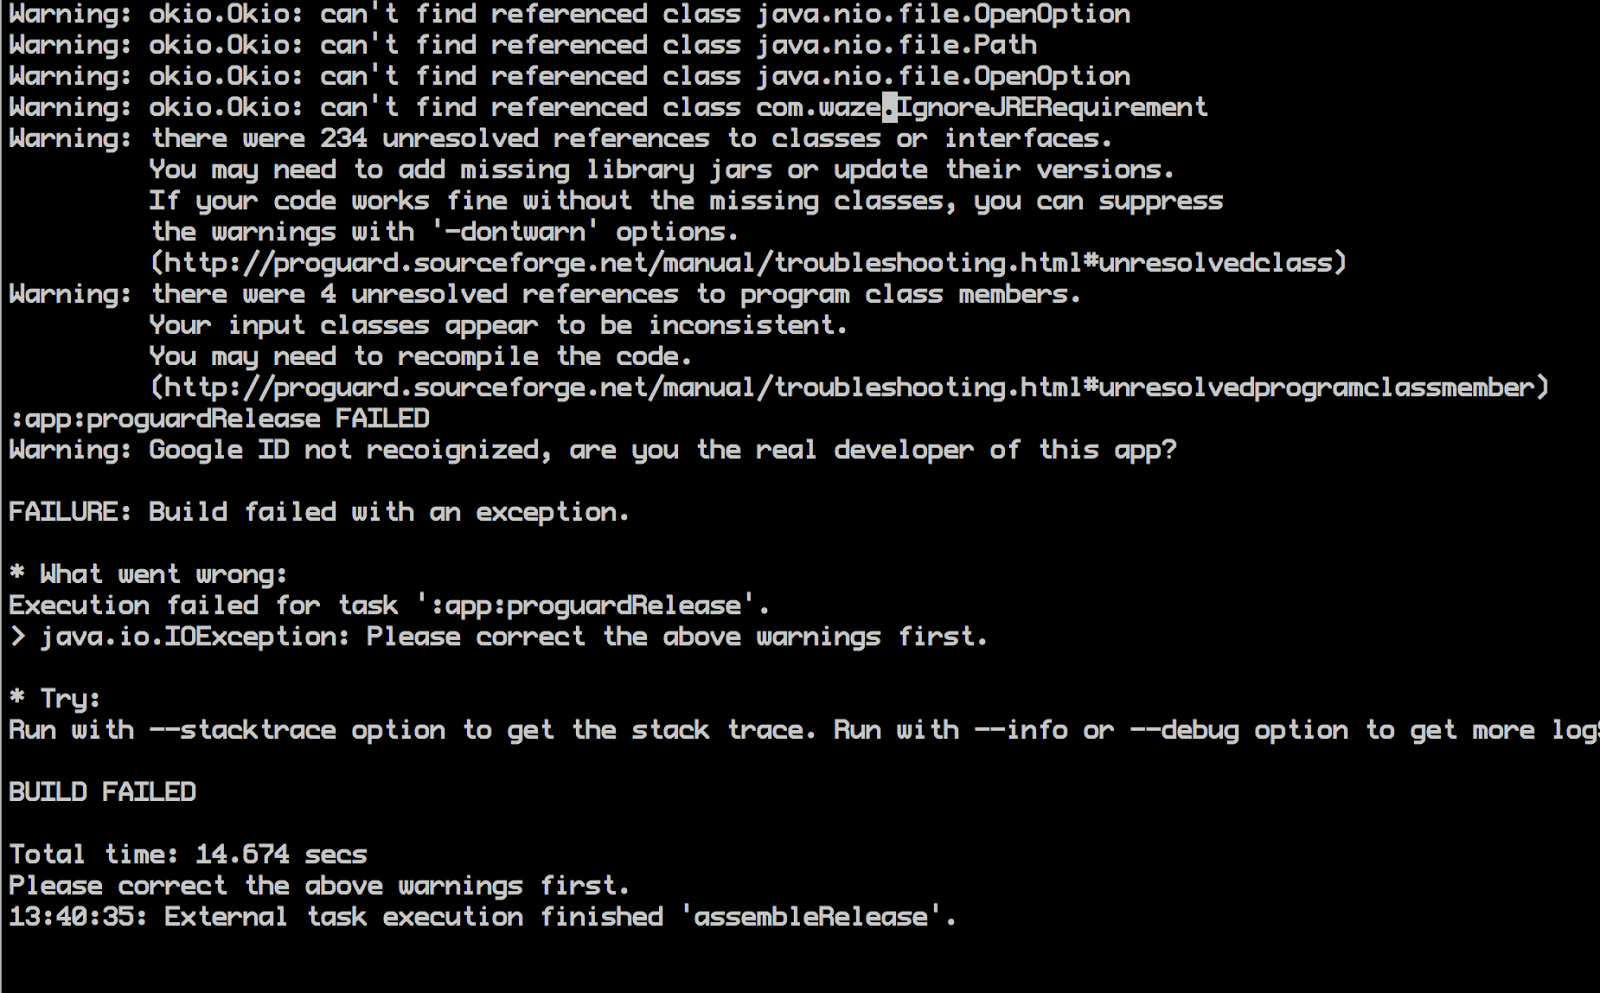
\includegraphics[width=0.6\textwidth]{imagenes/fig25.png}
    \caption{Error al intentar cambiar imagen}
  \end{center}
\end{figure}

ProGuard es una herramienta de compilación para Android. Ofusca, minimiza, optimiza y licencia el código de fuente para dificultar la ingeniería inversa en una aplicación. [1]